%%%%%%%%%%%%%%%%%%%%%%%%%%%%%%%%%%%%%%%%%%%%%%%%%%%%%%%
% Make sure to add any new macros to the final report 
% to ensure that they do not conflict with existsing
% ones.
%%%%%%%%%%%%%%%%%%%%%%%%%%%%%%%%%%%%%%%%%%%%%%%%%%%%%%%

\section{Reproduction of Results in the Paper}

Prior to applying the recent methods to new systems, we first explore their potential as inference algorithm for the rSLDS by reproducing the results of \cite{linderman_bayesian_2017}. We compare the Polyagamma approach to the variational inference algorithms by using data from an rSLDS that models the Synthetic NASCAR and solutions simulated from the chaotic Lorenz system.

\subsection{Synthetic NASCAR}

We generate a simulated dataset to represent a non-linear system that aims to imitate cars moving around a track. It consists of four states in total: two for driving along each straight section and two for navigating the semicircular turns at each end of the track. When constructing the rSLDS that models this dataset, we establish transition probabilities based solely on the preceding states. In other words, there is no reliance on the previous state $z_t$. Instead, each state is influenced by a constant bias $r_i$, which steers the transitions toward state $i$. This model is inherently less adaptable compared to the complete rSLDS formulation. Once we have created the rSLDS and generated a trajectory by sampling, we visualize the actual trajectory on a plot.
\begin{figure}[h!]
	\centering
	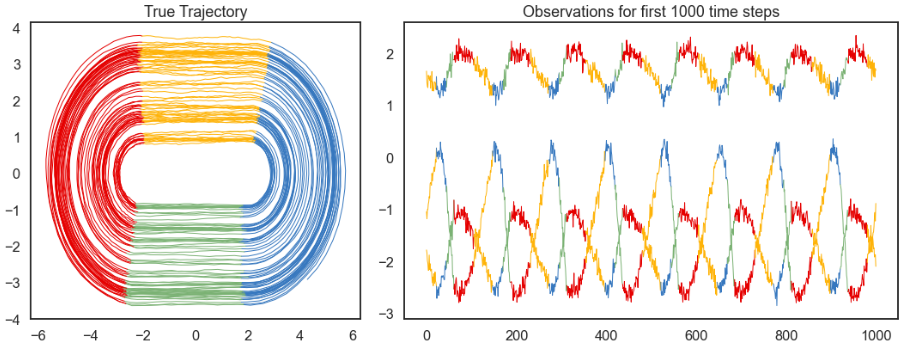
\includegraphics[width=0.75\textwidth]{paper_fig7.png}
	\caption{Exact trajectories of the Nascar model and the evolution of observations during the first 1000 time steps. The true dynamics switch between four states which are indicated by different colors.}
	\label{trueNascar}
\end{figure}

The left panel displays the continuous state trajectories, while the right one presents three observation traces from the first 1000 time steps. Although our observations have ten dimensions, we have plotted only three traces to maintain clarity and reduce visual clutter. Afterward, we proceed to create a new rSLDS object and train it using the data generated previously. It is important to note that this new rSLDS model will only have access to the observations, and it will not be aware of the true states or any other underlying information. By fitting and training the new model, we can recover the behavior of the system up to an affine transformation. The nonlinear behavior is learned by the model however one might still need to apply a rotation to recover the original vector field. This clarifies why the colors of the distinct states may not consistently correspond to the original ones. The behavior of NASCAR was simulated using both BBVI and Laplace EM methods, and the outcomes are presented in Figure \ref{generatedNascar}. It is evident that the estimated latent trajectories obtained through the Laplace EM method exhibit a closer match to the ground truth. Furthermore, the inferred trajectories by either of the variational algorithms demonstrate a closer alignment with the solution when compared to the Polyagamma approach.
\begin{figure}[h!]
	\centering
	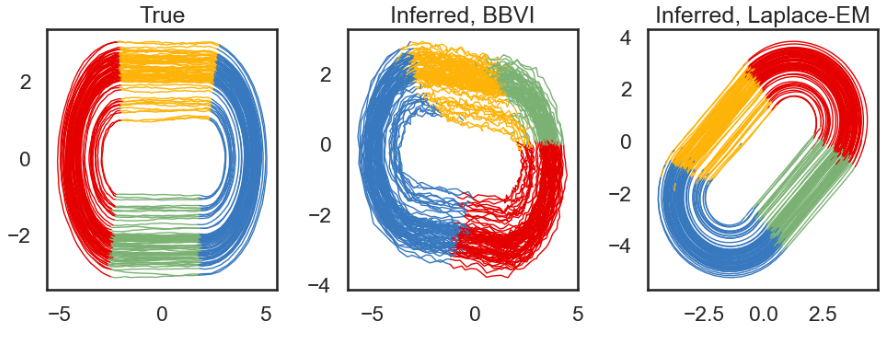
\includegraphics[width=0.75\textwidth]{paper_fig8.png}
	\caption{Generated trajectories of the Nascar model using rSLDS with both BBVI and Laplace EM.}
	\label{generatedNascar}
\end{figure}

\subsection{Lorenz system}
Rather than acquiring data from a linear model with Bernoulli observations, as stated in \cite{linderman_bayesian_2017}, we employ an ODE solver to generate data from a Lorenz system with various initial conditions. To enhance the realism of our data, we introduce perturbations by adding Gaussian noise with a mean of 0 and a variance of 1. We consider the resulting data as observations that would be utilized as input for our rSLDS model. Given the presence of two prominent states within the system, we construct our rSLDS model using 2 discrete states and a continuous latent variable of 3 dimensions. Subsequently, we fit the model to the 4-dimensional observations, and the outcomes for both the BBVI and Laplace EM approaches are condensed in Figure \ref{lorenz}. Regarding this system, both variational algorithms performed exceptionally well in inferring the qualitative behavior, and both yielded more accurate results compared to those discussed in \cite{linderman_bayesian_2017}.
\begin{figure}[h!]
	\centering
	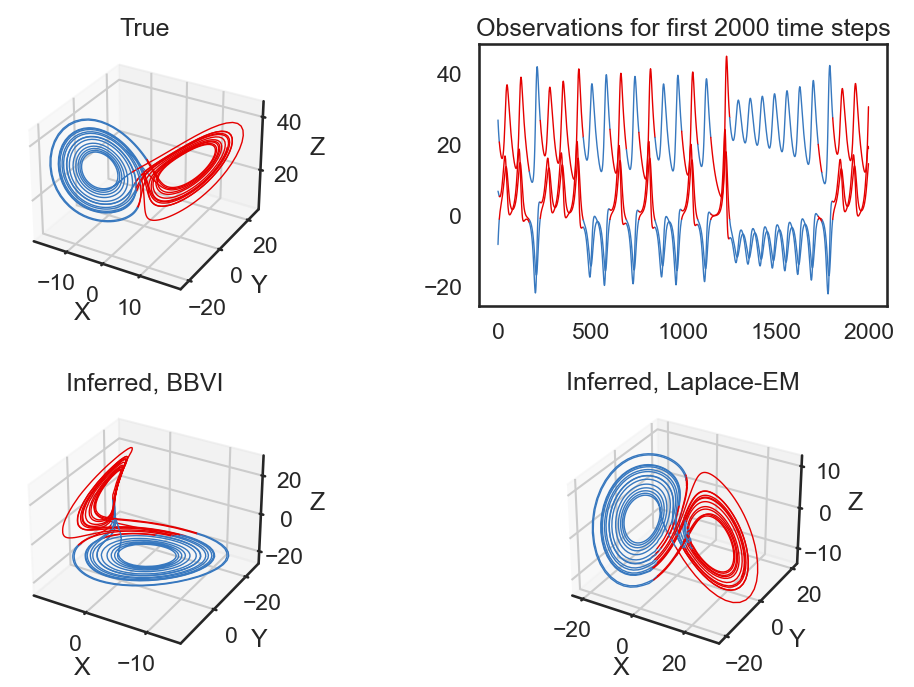
\includegraphics[width=0.75\textwidth]{paper_fig9.png}
	\caption{Qualitative behavior of the Lorenz system and comparison between true and generated states.}
	\label{lorenz}
\end{figure}
